%%%%%%%%%%%%%%%%%%%%%%%%%%%%%%%%%%%%%%%%%%%%%%%%%%%%%%%%%%%%%%%%%%%%%%%%%%%%%%%%
%2345678901234567890123456789012345678901234567890123456789012345678901234567890
%        1         2         3         4         5         6         7         8

\documentclass[letterpaper, 10 pt, conference]{ieeeconf}
\usepackage{graphicx}
\usepackage{amsmath}
\usepackage{gensymb}
\usepackage{relsize}
\usepackage{amsfonts}
\usepackage{mathtools}
\usepackage{lineno,amssymb,subcaption,algpseudocode,algorithm}
\usepackage[font={small}]{caption}
\usepackage{picins}

% Commands
\newcommand{\ubar}[1]{\text{\b{$#1$}}}
\DeclareMathOperator*{\minimize}{minimize}
\DeclareMathOperator*{\argmin}{argmin}
\DeclareMathOperator*{\subj}{subject\;to}
\DeclareMathOperator*{\st}{s.t.}

\newcommand{\cx}{\textsf{x}}
\newcommand{\cz}{\textsf{z}}
\newcommand{\cl}{\lambda}
\newcommand{\J}{\textsf{J}}
\newcommand{\cf}{\textsf{f}}
\newcommand{\cg}{\textsf{g}}
\newcommand{\ch}{\textsf{h}}
\newcommand{\X}{\textsf{X}}

\newlength\figwidth
\setlength\figwidth{\columnwidth}
\newlength\figheight
\setlength\figheight{5cm}

%\documentclass[a4paper, 10pt, conference]{ieeeconf}      % Use this line for a4 paper

\IEEEoverridecommandlockouts                              % This command is only needed if
                                                          % you want to use the \thanks command

\overrideIEEEmargins                                      % Needed to meet printer requirements.

% See the \addtolength command later in the file to balance the column lengths
% on the last page of the document

% The following packages can be found on http:\\www.ctan.org
%\usepackage{graphics} % for pdf, bitmapped graphics files
%\usepackage{epsfig} % for postscript graphics files
%\usepackage{mathptmx} % assumes new font selection scheme installed
%\usepackage{times} % assumes new font selection scheme installed
%\usepackage{amsmath} % assumes amsmath package installed
%\usepackage{amssymb}  % assumes amsmath package installed

\title{\LARGE \bf
Distributed model predictive control of multiple
vehicles transporting a flexible payload*
}


\author{Sampath Kumar Mulagaleti$^{1}$, Ruben Van Parys$^{1}$ and Goele Pipeleers$^{1}$%  <-this % stops a space
\thanks{*This work benefits from KU Leuven-BOF PFV/10/002 Centre of Excellence: Optimization in Engineering (OPTEC); from the Belgian Programme on Interuniversity Attraction Poles, initiated by the Belgian Federal Science Policy Office (DYSCO); from the project G0C4515N of the Research Foundation-Flanders (FWO-Flanders); and from the KU Leuven Research project C14/15/067. Ruben Van Parys is a PhD fellow of FWO-Flanders. }%
\thanks{$^{1}$The authors are with the MECO Research Group, Department of Mechanical Engineering, Division PMA, KU Leuven, 3001 Leuven, Belgium and are member of Flanders Make. \texttt{sampath.kumar.mulagaleti@gmail.com}}
}

\begin{document}



\maketitle
\thispagestyle{empty}
\pagestyle{empty}


%%%%%%%%%%%%%%%%%%%%%%%%%%%%%%%%%%%%%%%%%%%%%%%%%%%%%%%%%%%%%%%%%%%%%%%%%%%%%%%%
\begin{abstract}
This paper presents a strategy for the control of multiple vehicles that cooperatively transport a flexible payload. To this end, an algorithm is developed which generates optimal trajectories for the vehicles to follow. Solving an optimization problem composes the core of the algorithm. The problem is first decomposed over the vehicles using the Alternating Direction Method of Multipliers (ADMM) algorithm. This results in each vehicle solving a sub-problem to generate its own optimal trajectory. The algorithm instructs that the optimization problem be solved repeatedly in a receding horizon fashion, making it fit into a distributed model predictive control (DMPC) framework. One ADMM iteration is performed per DMPC iteration, reducing the inter-agent communication rate. Numerical validation of the developed control scheme is performed and the results are presented.
\end{abstract}


%%%%%%%%%%%%%%%%%%%%%%%%%%%%%%%%%%%%%%%%%%%%%%%%%%%%%%%%%%%%%%%%%%%%%%%%%%%%%%%%
\section{INTRODUCTION}

Payload transportation tasks are ubiquitous in industrial environments. These payloads can vary greatly in weights, necessitating multiple transportation solutions of different payload capacities within the same logistics structure. An alternative to this would be to use multiple vehicles to cooperatively tow a payload, with the number of vehicles chosen according to the towing requirements. To enable such a multi-agent system to work autonomously and transport the payload to a desired location, control strategies are required which perform coordinated motion of the vehicles.
\\
\indent Transportation of objects with multiple vehicles is a standard problem in robotics and control. Some of the early approaches to model and control such systems are presented in \cite{c1,c2,c3}, and an optimal control approach in \cite{c4}. More recent approaches utilize a Model Predictive Control (MPC) framework, which allows to explicity incorporate system constraints in the optimization problem. Such techniques have been applied to perform trajectory tracking with multiple vehicles moving in a desired formation \cite{c5}. Motion planning for multiple vehicles moving in a formation is done within a receding horizon framework in \cite{c6}, utilizing a leader-follower strategy. Such a strategy is not robust against possible failure of the leader agent. This necessitates development of strategies in which each agent has equal role to play within the multi-agent system. This leads to the domain of Distributed model predictive control (DMPC). Within the DMPC framework, the control problem is distributed over the agents. Since an optimization problem underlies the MPC framework, DMPC based techniques usually utilize distributed optimization methods to distribute the optimization problem over the agents \cite{c7}. Motion planning algorithms are designed within this framework in \cite{c8} and \cite{c9} for formation control of multiple agents.
\\
\indent
 A major difference between formation control problems and the payload transportation problem is that in the latter, the agents are dynamically coupled. This means that a change in state of one of the agents results in a change in state of the others. The coupled dynamics act as constraints on the centralized optimization problem, and decomposing the centralized problem for DMPC purposes would require decomposing the coupling dynamics constraint. Decoupling of dynamics is done using primal decomposition
 in \cite{c10}, in which, linear systems are considered, and an optimal consensus problem is solved. In optimal consensus problems, multiple optimization variables are driven to the
 same value over iterations. In other words, consensus is achieved between different states of the system. Another approach based on dual decomposition, is discussed in \cite{c11}. In this, the variable splitting method is employed \cite{c8}, with the introduction of copies of states of neighboring vehicles which affect local states of a host vehicle. More robust methods based on the ADMM are formulated in \cite{c12}, which consider coupled objective functions in addition to coupled nonlinear dynamics. Another alternative is introduced in \cite{c13}, where the
 ADMM-consensus problem introduced in \cite{c14} is combined with the idea of introducing copies of neighboring states from \cite{c11}.
 \\
 \indent
 This work proposes a decentralized-consensus ADMM based DMPC scheme to solve the cooperative payload transportation problem. Decentralized-consensus is achieved by decoupling the 2nd ADMM step using a novel variable-copying scheme inspired from \cite{c9}. In order to reduce the communication and computation load, 1 ADMM iteration is performed per DMPC iteration, and the ADMM iterations are supported by inter-vehicle communication.
 \\ \\ \indent
 The rest of the paper is organized as follows: \\
Section  II  introduces  the  motion  planning  problem  for
cooperative payload transportation problem, and Section III describes how
this  problem  can  be  solved  in  a  online distributed manner. Results from simulations based on the proposed approach are presented in Section IV, and the results from an experimental validation in Section V.
\section{PROBLEM FORMULATION}
\subsection{System model}
The dynamic system under consideration is modeled as multiple holonomic vehicles attached through 1D spring-damper elements to a common payload. The payload and the holonomic vehicles are abstracted as point masses, and are constrained to move in a 2D plane. Dynamic spring-mass-damper models are used to describe the system in the optimization problem. Friction is ignored in the model. The free length of the flexible elements is assumed to be $0$ m, resulting in the vehicles only applying a pulling force on the payload. A schematic of this model for 3 holonomic vehicles is shown in \ref{2D_schematic}.

\begin{figure}
  \centering
  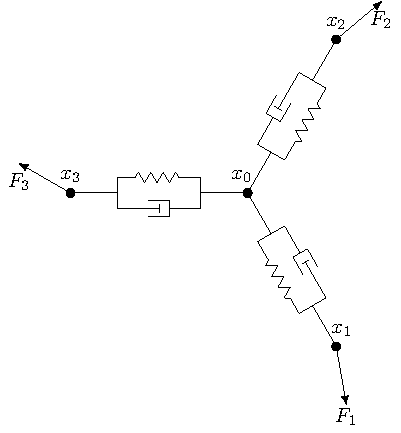
\includegraphics[scale=1]{figures/schematic.pdf}
  \caption{Dynamic model decoupling}
  \label{2D_schematic}
\end{figure}

\subsection{Optimal control problem}
This section discusses the formulation of optimization problem with the payload and vehicle trajectories as the optimization variables. The solution of this problem are the position trajectories the vehicles and the payload should follow in order to transport the payload to a location closest to its goal $x_d \in \mathbb{R}^2$ within the time horizon $T$ \textit{s} over which the problem is solved.
The payload trajectory is represented by the vector ${x_0(t) \in \mathbb{R}^2}$ and that of each vehicle $i$ by ${x_i(t) \in \mathbb{R}^2}$.
 The formulation is shown in \eqref{label:central}. The case of $N$=3 vehicles is dealt here. Extension to problems with more vehicles can be done by modifying the \textit{intra-vehicle anti-collision} constraints.

\begin{equation}
  \label{label:central}
  \begin{aligned}
    & \minimize_{\forall i:x_i(t),x_0(t)} && \mathlarger{\int_0^T} \mathlarger{||}x_0(t)-x_d\mathlarger{||}_1 dt \\
    & \subj
    && \ubar{l} \preceq f_i(x_0(t),x_i(t)) \preceq \bar{l}\\
    &       && g(x_0(t),x_1(t),x_2(t),x_3(t)) = 0 \\
    &        && h_{ij}(x_0(t),x_i(t),x_j(t)) \leq 0 \\
    &        && \ubar{d} \leq d_i(x_i(t)) \leq \bar{d} \\
    &       && x_0^{(k)}(0) = x_{0,0}^{(k)}, \quad x_i^{(k)}(0) = x_{0,i}^{(k)} \\
       &       && x_0^{(k)}(T) = x_{T,0}^{(k)} , \quad x_i^{(k)}(T) = x_{T,i}^{(k)} \\
       &       && k\in{0,1,2} \\
    &                                && \forall t \in [0,T], \quad \forall i,j \in \{1,2,3\}, i \neq j
  \end{aligned}
\end{equation}
The function $f_i:\mathbb{R}^4\to\mathbb{R}^3$ consists of individual vehicle $i$'s dynamics, and flexible element $i$'s length. The lower and upper bounds on these quantities are captured in vectors $\ubar{l}$ and $\bar{l}$ respectively. The function $g:\mathbb{R}^8\to\mathbb{R}$ represents the payload dynamics.
\\
 Intra-vehicle collisions are avoided using the third constraint, defined by the function $h_{ij}:\mathbb{R}^6\to\mathbb{R}$. It limits the angles between the vehicles to lie at greater than 90$\degree$ when subtended at the payload. It is reiterated that for $N$$>$$3$, this constraint should be reformulated.
 These functions are shown in \eqref{eq:cons}. Note that the indication of time dependence of the variables is dropped for ease of notation.

 \begin{equation}\label{eq:cons}
 \begin{aligned}
 f_i(x_0,x_i) &=
 \begin{bmatrix}
   m_i\ddot{x}_i + c_i(\dot{x}_i-\dot{x}_0) + k_i(x_i-x_0) \\
  (x_i-x_0)^T(x_i-x_0)
 \end{bmatrix} \\
 g(x_0,x_1,x_2,x_3) &= m_0\ddot{x}_0 +  \sum\limits_{i=1}^{3}
 \begin{bmatrix}{c_i(\dot{x}_i-\dot{x}_0) + k_i(x_i - x_0)} \end{bmatrix}\\
 h_{ij}(x_0(t),x_i(t),x_j(t)) &= \mathlarger{\langle} x_i(t) - x_0(t),x_j(t) - x_0(t) \mathlarger{\rangle}
 \end{aligned}
 \end{equation}
 The rest of the constraints represent limits on vehicle velocities and accelerations, and initial and final conditions on the vehicle and payload position trajectories and higher derivatives.
\section{Solution strategy}
\subsection{Spline parameterization}
Problem \eqref{label:central} represents an infinite dimensional problem, since the optimization variables $x_0(t)$ and $x_i(t)$ are infinite dimensional, and enforcing the constraints at all instances results in an infinite number of constraints. In order to make the problem numerically tractable, a B-spline based parameterization of the optimization variables is used, along the lines of \cite{c15}. The continuous optimization variables are hence represented as linear combinations of piecewise polynomial basis functions $b_k(t)$, as expressed in \eqref{spline}.

\begin{equation}\label{spline}
x_i(t) = \sum\limits_{k=1}^{n} \cx_{i,k}b_k(t) = \cx_i^Tb(t) \quad \forall i \in \{1,.,N\}
\end{equation}

 The trajectories of each vehicle $i$ are consequently represented by the coefficient set $\cx_i$$=$ $\{\cx_{i,k}\}_{k=1}^{n}$ and those of the payload by $\cx_0$$=$$\{\cx_{0,k}\}_{k=1}^{n}$, for a chosen B-spline basis functions vector $b = [b_1,\ldots,b_n]^T$. Substituting these parameterizations in \eqref{label:central} results in an optimization problem with finite number of variables. A B-spline parameterization is chosen because of its convex hull property \cite{c15}, which dictates that the resultant spline function lies within the convex hull of the coefficients. This is because at every time instant over which the spline is defined, the basis functions correspond to a non-negative partition of unity. Hence, the constraints on an infinite dimensional spline can be imposed on the coefficients of the corresponding B-spline basis functions, resulting in a finite number of constraints. Since the constraint functions $f_i$,$g$ and $h_{ij}$ are composed of polynomial combinations of the splines $x_i(t)$ and $x_0(t)$ and their derivatives, the resultant splines' coefficients are polynomial combinations of $\cx_0$ and $\cx_i$. Following the convex hull property, these constraints are transformed to $\cf_i$,$\cg$ and $\ch_{ij}$ respectively.
The resultant formulation is seen in \eqref{withparam}.

 \begin{equation}
   \label{withparam}
   \begin{aligned}
     & \minimize_{\forall i:\cx_i,\cx_0} &&  \J(\cx_0) \\
     & \subj
     && \ubar{l} \preceq \cf_i(\cx_0,\cx_i) \preceq \bar{l}\\
     &       && \cg(\cx_0,\cx_1,\cx_2,\cx_3) = 0 \\
     &        && \ch_{ij}(\cx_0,\cx_i,\cx_j) \leq 0 \\
     &        && \cx_i \in \X_i \\
     &        && \cx_0 \in \X_0 \\
     &                                && \forall i,j \in \{1,2,3\}, i \neq j
   \end{aligned}
 \end{equation}
 The MPC updating scheme proposed in \cite{c16} for optimization variables expressed in a B-spline basis can be used on a centralized processor, provided it has access to all $\cx_i$ and $\cx_0$ variables. This scheme is reiterated in Algorithm~\ref{alg:mpc}. The vehicle and payload positions estimated at time $(k+1)\Delta T$ are incorporated into the feasible sets $\X_i$ and $\X_0$ while solving the problem for $\cx_i^{k+1}$ and $\cx_0^{k+1}$.

 \algblockdefx[Name]{Repeat}{Until}[1][Unknown]{\textbf{Repeat} #1}{\textbf{Until }}
 \begin{algorithm}[t]
 \caption{Spline-based MPC}\label{alg:mpc}
 \begin{algorithmic}[1]
 \Repeat[every $\Delta T$:  $k=0,1,\ldots$]
   \State Extract $x_i^k(t)$ from $\cx_i^k$ for each Vehicle $i$.
   \State Vehicle $i$ starts following trajectory $x_i^k(t)$
   \State Estimate $\hat{x}_i^k$ and $\hat{x}_0^k$ at time $(k+1)\Delta T$
   \State Compute $\cx_i^{k+1}$ and $\cx_0^{k+1}$ by solving \eqref{withparam}, using $\hat{x}_i^k$, $\hat{x}_0^k$ as initial conditions and hot start coefficients
 \Until target reached
 \end{algorithmic}
 \end{algorithm}


 \subsection{Distributed formulation}
 The purpose of this section is to split the optimization problem \eqref{withparam} into 3 separate problems, one for each vehicle. This means that each problem should contain optimization variables local to the vehicle it is assigned. The first step towards the distributed formulation is the introduction of copies of the payload variables $\cx_0$ on each vehicle. These variables are represented by $\cx_{i0}$. The substitution of these variables results in 3 copies of the payload dynamics constraint $\cg$, each one being $\cg_i(\cx_{i0},\cx_i,\cx_j) = 0$, where $\cx_j = \{\cx_1,\cx_2,\cx_3\}\ominus \cx_i$.
 \\ \indent
 The payload dynamics constraint is further decoupled by borrowing ideas from \cite{c11}, which dictates that the variables $x_{j}(t)$ of vehicle $j$ which affect the dynamics of vehicle $i$ can be modeled as exogenous inputs $x_{ij}(t)$ acting on vehicle $i$. The new variables $x_{ij}(t)$ are hence local to vehicle $i$, and are parameterized by the spline coefficients $\cx_{ij}$. The payload dynamics constraint is thus further modified as $\cg_i(\cx_{i0},\cx_i,\cx_{ij}) = 0$. This substitution is supported by consensus constraints between  $\cx_{j}$ and $\cx_{ij}$. Following a modification of the consensus constraints presented in \cite{c9}, consensus variables $\cz_{ij}$ are introduced on each vehicle $i$, which act as a balance between $\cx_{j}$ and $\cx_{ij}$. The modified optimization problem with local copy variables, consensus variables, and consensus constraints is shown in \eqref{main_problem}.
   \begin{equation}
     \label{main_problem}
     \begin{aligned}
       & \minimize_{\forall i,j,i \neq j:\cx_i,\cx_{ij},\cz_{ij},\cx_{i0}} &&  \sum\limits_{i=1}^{3}\J(\cx_{i0}) \\
       & \subj
       && \ubar{l} \preceq \cf_i(\cx_{i0},\cx_i) \preceq \bar{l}\\
       &       && \cg_i(\cx_{i0},\cx_i,\cx_{ij}) = 0 \\
       &        && \ch_{ij}(\cx_{i0},\cx_i,\cx_{ij}) \leq 0 \\
       &         && \cx_{ij} = \cz_{ij},\, \cx_{j} = \cz_{ij} \\
       &        && \cx_i \in \X_i,\, \cx_{i0} \in \X_0 \\
       &                                && \forall i,j \in \{1,2,3\}, i \neq j
     \end{aligned}
   \end{equation}

  \indent
 The optimization problem \eqref{main_problem} can now be decoupled using the Alternating Direction Method of Multipliers (ADMM). The ADMM algorithm solves the dual of \eqref{main_problem}, after augumenting it with a quadratic term to improve convergence properties. To minimize duality gap, the fewest number of constraints are to be dualized according to \cite{c8}. Hence, only the consensus equality constraints are moved into the objective function to form the lagrangian. This appended objective function is seen in \eqref{Lagrangian}.


 \begin{equation}\label{Lagrangian}
   \begin{aligned}
   \mathcal{L}_\rho &=
  {\mathlarger{\sum\limits_{i=1}^{N}}}
  {\mathlarger{\mathlarger{(}}}\J_i(\cx_{i0}) +
 \mathlarger{\sum\limits_{j \neq i}} \mathlarger{(} \lambda_{ij}^T(\cx_{ij} - \cz_{ij}) + \cfrac{\rho}{2} \mathlarger{||}\cx_{ij} - \cz_{ij}\mathlarger{||}_2^2{{\mathlarger{)}}} \\ & \qquad \qquad \qquad \qquad
  + \mathlarger{\sum\limits_{j \neq i}} \mathlarger{(} \mu_{ij}^T(\cx_{j} - \cz_{ij}) +
   \cfrac{\rho}{2} \mathlarger{||}\cx_{j} - \cz_{ij}\mathlarger{||}_2^2 \mathlarger{)}\mathlarger{\mathlarger{\mathlarger{)}}}
   \\
   &= {\mathlarger{\sum\limits_{i=1}^{N}}}  \mathcal{L}_{\rho,i} (\cx_{i0},\cx_{ij},\cz_{ij},\lambda_{ij},\cx_{j},\mu_{ij}) \\
   &= {\mathlarger{\sum\limits_{i=1}^{N}}}  \mathcal{L}_{\rho,i} (\cx_{i0},\cx_{ij},\cz_{ij},\lambda_{ij},\cx_{i},\cz_{ji},\mu_{ji})
   \end{aligned}
   \end{equation}
The dual variables introduced in the Lagrangian corresponding to the equality constraints are $\lambda_{ij}$ and $\mu_{ij}$. The last equality in \eqref{Lagrangian} is valid due to the bidirectionality of interaction amongst the vehicles: variables on vehicle $i$ affecting the dynamics of vehicle $j$ correspond to the variables on vehicle $j$ affecting dynamics of vehicle $i$.
Since the constraints are now completely decoupled, the feasible set on each vehicle $i$ is represented by $\{\cx_{i},\cx_{i0},\cx_{ij}\} \in \Phi_i$. The dual function of \eqref{main_problem} is shown in \eqref{dual_problem}.
\begin{equation}\label{dual_problem}
q(\lambda_{ij},\mu_{ij}) = \inf_{\substack{\{\cx_{i},\cx_{i0},\cx_{ij}\} \in \Phi_i \\ \forall i,j \in \{1,2,3\}, i \neq j}} \mathcal{L}_{\rho}\
\end{equation}

The dual variables are found by maximizing the dual function $q$ with respect to the lagrangian multipliers. The maximization is performed through gradient ascent in the ADMM algorithm. For this, the primal variables $\cx_{ij}^k$,$\cx_{j}^k$ and $\cz_{ij}^k$ from iteration $k$ are updated in iteration $k+1$, and the gradient of the dual function $q$ is calculated in the directions of the lagrangian multipliers according to \eqref{gradients}.
\begin{equation}\label{gradients}
  \begin{aligned}
    \nabla_{\lambda_{ij}} q    &= \cx_{ij}^{k+1} - \cz_{ij}^{k+1}\\
    \nabla_{\mu_{ij}} q &= \cx_{j}^{k+1} - \cz_{ij}^{k+1}
  \end{aligned}
\end{equation}
 An optimal step of length $\rho$ in these directions is taken. The primal variables are updated in two steps in a Gauss-Siedel fashion, the first step updating the $\{\cx_{i},\cx_{i0},\cx_{ij}\}$ variables and the second updating the $\cz_{ij}$ variables.
\\
\indent
Solving the optimization problem \eqref{withparam} till convergence will require several ADMM iterations. These iterations will replace~(step 5) in Algorithm~\ref{alg:mpc}, and would be performed on individual vehicles in parallel. However, this would also result in a substantial computation and communication load for each MPC iteration. This is avoided by following the DMPC scheme proposed in \cite{c16}, which performs 1 ADMM iteration per MPC iteration. The resultant is Algorithm~\ref{alg:dmpc}, which includes the communication steps performed in one DMPC iteration.
\algblockdefx[Name]{Repeat}{Until}[1][Unknown]{\textbf{Repeat} #1}{\textbf{Until }}
\begin{algorithm}[t]
\caption{ADMM based Distributed MPC}\label{alg:dmpc}
\begin{algorithmic}[1]
\State Perform $n$ ADMM iterations and get $\cx_i^0$, $\cx_{ij}^0$, $\cx_{i0}^0$, $\cz_{ij}^0$, $\lambda_{ij}^0$, $\mu_{ij}^0$
\Repeat[every $\Delta T$:  $k=0,1,\ldots$]
  \State Extract $x_i^k(t)$, $x_{ij}^k(t)$ and $x_{i0}^k(t)$ from $\cx_i^k$, $\cx_{ij}^k$ and $\cx_{i0}^k$ \hspace{2.8cm} on each Vehicle $i$.
  \State Vehicle $i$ starts following trajectory $x_i^k(t)$
  \State Estimate $\hat{x}_i^k$ and $\hat{x}_{i0}^k$ at time $(k+1)\Delta T$, assuming perfect tracking of $x_{ij}^k(t)$
  \State Update horizon and compute $\tilde{\cx}_i^k$, $\tilde{\cx}_{ij}^k$, $\tilde{\cx}_{i0}^k$, $\tilde{\cz}_{ij}^k$,
  $\tilde{\cz}_{ji}^k$, $\tilde{\lambda}_{ij}^k$, $\tilde{\mu}_{ji}^k$
  \State \label{xupdate_rh} Compute $\{\cx_i^{k+1},\cx_{ij}^{k+1},\cx_{i0}^{k+1}\}$, using $\hat{x}_i^k$ and $\hat{x}_{i0}^k$ as initial conditions:
  \small
  \begin{align*}
  \left(\begin{matrix}\cx_i^{k+1} \\[0.5em] \cx_{ij}^{k+1} \\[0.5em] \cx_{i0}^{k+1} \end{matrix} \right) &:=
    \argmin\limits_{\{\cx_{i},\cx_{i0},\cx_{ij}\} \in \Phi_i}\mathcal{L}_{\rho,i} (\cx_{i0},\cx_{ij},\tilde{\cz}^k_{ij},\tilde{\lambda}^k_{ij},\cx_{i},\tilde{\cz}^k_{ji},\tilde{\mu}^k_{ji})
  \intertext{\normalsize
  \State Communication with agents j:\ :
  \Statex \hspace{0.8cm} send $\cx_i^{k+1}$, receive $\cx_j^{k+1}$
  \State Compute $\cz_{ij}^{k+1}$:
  }
  \cz_{ij}^{k+1} &:= \cfrac{1}{2}\left(\cx^{k+1}_{j}+\cx^{k+1}_{ij}+\cfrac{\tilde{\lambda}^{k}_{ij}+\tilde{\mu}^{k}_{ij}}{\rho}\right)
  \intertext{\normalsize
  \State Compute $\lambda_{ij}^{k+1}$ and $\mu_{ij}^{k+1}$:
  }
  \lambda_{ij}^{k+1}  &:=  \tilde{\lambda}_{ij}^{k} + \rho (\cx_{ij}^{k+1} - \cz_{ij}^{k+1}) \\
  \mu_{ij}^{k+1}  &:=  \tilde{\mu}_{ij}^{k} + \rho (\cx_{j}^{k+1} - \cz_{ij}^{k+1})
  \end{align*}
  \normalsize
  \State Communication with agents $j\:$
  \Statex \hspace{0.8cm} send $\cz_{ij}^{k+1}$ and $\mu_{ij}^{k+1}$, receive $\cz_{ji}^{k+1}$ and $\mu_{ji}^{k+1}$
\Until target reached
\end{algorithmic}
\end{algorithm}
\\
\indent
The algorithm dictates that first, a few ADMM iterations be performed to find the first set of primal and dual variables. The primal $\cx_{i}$ variables are then interpreted in terms of the trajectories $x_i(t)$ on each vehicle $i$, and the tracking of these trajectories begins. According to the spline-MPC scheme discussed in \cite{c16}, $\hat{x}_i(\Delta T)$ and $\hat{x}_{i0}(\Delta T)$ are estimated locally on each vehicle, with perfectly tracked $x_{ij}(t)$ as the exogenous inputs into the local model. These estimates are passed as initial conditions into the MPC problem solving the trajectories from time $\Delta T$ s. This is followed by the usual 3 ADMM steps, with steps 7 and 9 for calculating the primal variables, and 10 for the dual variables. Since variables from the previous ADMM iteration are used in the current iteration, the spline coefficients are transformed to represent the spline in the current time frame, as discussed in \cite{c16}. Step 6 of the algorithm deals with this transformation. Step 9 is the direct least squares solution of the second ADMM step to update the $\cz_{ij}$ variables, and the corresponding problem is shown in \eqref{z_step}.
\begin{equation}
\label{z_step}
\begin{aligned} \cz_{ij}^{k+1} &:=
 \argmin_{\cz_{ij}} \quad (\tilde{\lambda}^k_{ij})^T(\cx^{k+1}_{ij} - \cz_{ij}) + \cfrac{\rho}{2} \mathlarger{||}\cx^{k+1}_{ij} - \cz_{ij}\mathlarger{||}_2^2{{}} \\ & \qquad \qquad \qquad \qquad
+ (\tilde{\mu}^k_{ij})^T(\cx^{k+1}_{j} - \cz_{ij}) +
\cfrac{\rho}{2} \mathlarger{||}\cx^{k+1}_{j} - \cz_{ij}\mathlarger{||}_2^2 \mathlarger{}
\end{aligned}
\end{equation}
\\
\indent
From this least squares problem, it can be seen the consensus variables $\cz_{ij}$ are pushed between the \textit{expected} $\cx_{ij}$ variables and the \textit{actual} $\cx_j$ variables, acting as a balance between them. In the first ADMM step (Step 7), the reverse occurs in that $\cx_{ij}$ and $\cx_j$ are pushed towards the previous \textit{compromise} $\cz_{ij}$ variables. Thus, over MPC (and hence, ADMM) iterations, a consensus is achieved between $\cx_{ij}$ and $\cx_j$, resulting the problem dynamics being satisfied.



\begin{thebibliography}{99}

\bibitem{c1} D. Williams and O. Khatib, "The virtual linkage: a model for internal forces in multi-grasp manipulation," [1993] Proceedings IEEE International Conference on Robotics and Automation, Atlanta, GA, 1993, pp. 1025-1030 vol.1.
doi: 10.1109/ROBOT.1993.292110
\bibitem{c2}O. Khatib. Force strategies for cooperative tasks in multiple mobile manipulation
systems. Giralt G., Hirzinger G. (eds) Robotics Research. Springer, London, 1996.
\bibitem{c3}H. G. Tanner, K. J. Kyriakopoulos, and N. J. Krikelis. Modeling of multiple mobile
manipulators handling a common deformable object. Journal of Robotic Systems,
15(11):599?623, 1998.
\bibitem{c4}R. Ritz and R. D?Andrea. Carrying a flexible payload with multiple flying vehicles.
In 2013 IEEE/RSJ International Conference on Intelligent Robots and Systems, pages
3465?3471, Nov 2013.
\bibitem{c5}S. Liu, D. Sun, and C. Zhu. Coordinated motion planning for multiple mobile robots
along designed paths with formation requirement. IEEE/ASME Transactions on
Mechatronics, 16(6):1021?1031, Dec 2011.
\bibitem{c6} M. Saska, V. Von ?
asek, T. Krajn ??k, L. P?reu?
cil, Coordination
and navigation of heterogeneous mav?ugv formations localized
by a hawk-eye-like approach under a model predictive control
scheme, The International Journal of Robotics Research 33 (10)
(2014) 1393?1412.
\bibitem{c7} S. Boyd, L. Xiao, and A. Mutapcic. Notes on decomposition methods, October 2003.
\bibitem{c8} R. L. Raffard, C. J. Tomlin, and S. P. Boyd. Distributed optimization for cooperative
agents: application to formation flight. In 2004 43rd IEEE Conference on Decision
and Control (CDC) (IEEE Cat. No.04CH37601), volume 3, pages 2453?2459 Vol.3, Dec
2004.
\bibitem{c9} R. V. Parys and G. Pipeleers. Online distributed motion planning for multi-vehicle
systems. In 2016 European Control Conference (ECC), pages 1580?1585, June 2016.
\bibitem{c10} B. Johansson, A. Speranzon, M. Johansson, and K. H. Johansson. On decentralized
negotiation of optimal consensus. Automatica, 44(4):1175 ? 1179, 2008.
\bibitem{c11} P. Giselsson and A. Rantzer. Distributed model predictive control with suboptimality
and stability guarantees. In 49th IEEE Conference on Decision and Control. pp.
7272-7277.
\bibitem{c12} F. Farokhi, I. Shames, and K. H. Johansson. Distributed MPC Via Dual Decompo-
sition and Alternative Direction Method of Multipliers, pages 115?131. Springer
Netherlands, Dordrecht, 2014.
\bibitem{c13} T. H. Summers and J. Lygeros. Distributed model predictive consensus via the
alternating direction method of multipliers. In 2012 50th Annual Allerton Conference
on Communication, Control, and Computing (Allerton), pages 79?84, Oct 2012.
\bibitem{c14} S. Boyd, N. Parikh, E. Chu, B. Peleato, and J. Eckstein. Distributed optimization and
statistical learning via the alternating direction method of multipliers. Found. Trends
Mach. Learn., 3(1):1?122, Jan. 2011.
\bibitem{c15} W. Van Loock, G. Pipeleers, J. Swevers, B-spline parameterized
optimal motion trajectories for robotic systems with guaranteed constraint satisfaction, Mechanical Sciences 6 (2) (2015) 163-171.
\bibitem{c16} Ruben Van Parys, Goele Pipeleers, Distributed MPC for multi-vehicle systems moving in formation, In Robotics and Autonomous Systems, Volume 97, 2017, Pages 144-152, ISSN 0921-8890, https://doi.org/10.1016/j.robot.2017.08.009.
\end{thebibliography}%
\end{document}